% !TEX root = ../main.tex
\section{Preprocessing and Validation of Collected Data} \label{sec:preprocessvalidate}

  

	\subsection{Preprocessing of Data}
		\todo[inline, color=blue!60]{Skrive litt om hvordan jeg har håndtert rådata. Hvilke verdier er inkludert, hvilke er utelukket, osv. Litt om tomme svar, etc.}

    \begin{figure}[H]
      \centering
      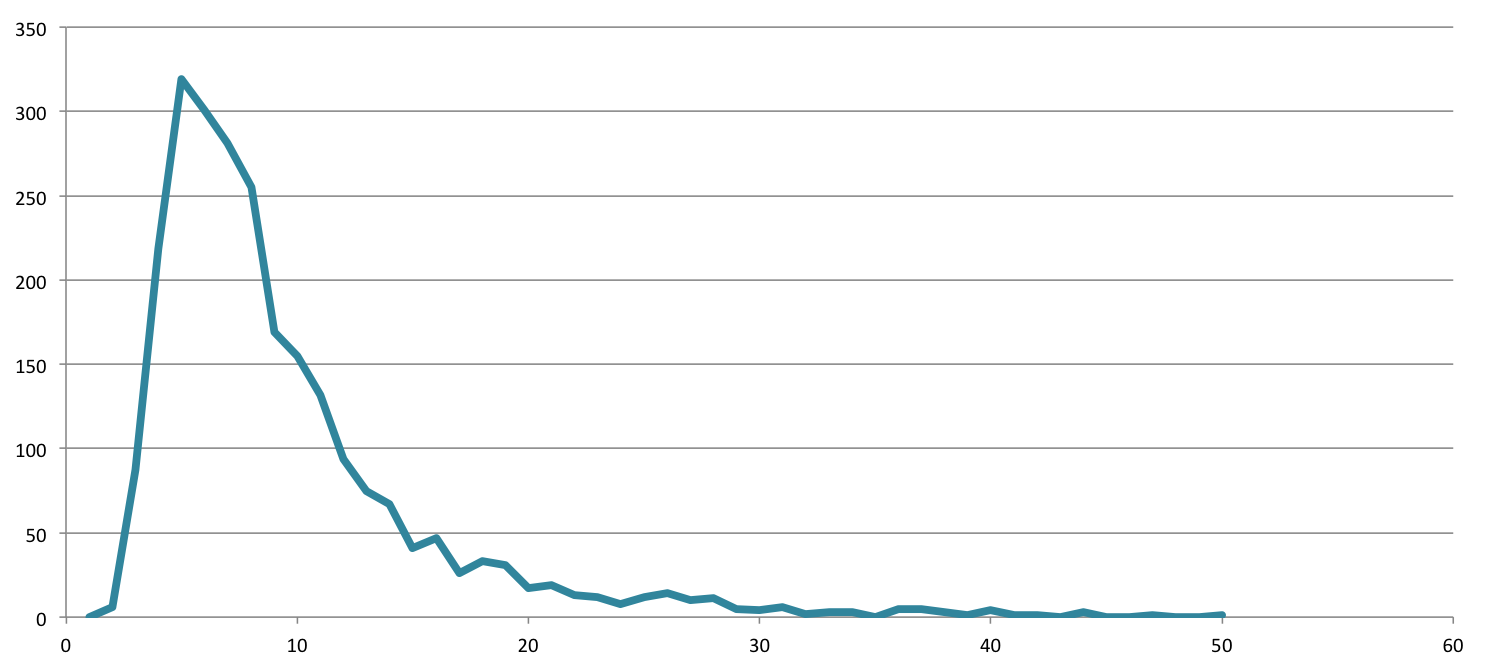
\includegraphics[width=\textwidth]{pics/analysis/limittimeframe.png}
      \caption{Defining max pattern creation time}
    \end{figure}

	\subsection{The Impact of Using Latin Square} \label{sec:latinsquareimpact}

    \todo[inline, color=orange!80]{Se om rekkefølge på mønster har noe å si}

		%Figure: Percentage of times the pattern orders occurred
		\begin{figure}[H]
      \centering
      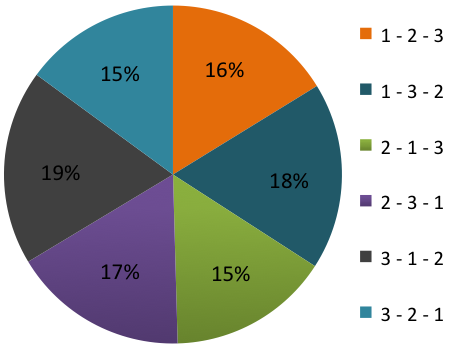
\includegraphics[scale=0.5]{pics/analysis/patternOrder.png}
      \caption{Percentage of times the pattern orders occurred}
      \label{fig:patternOrder}
    \end{figure}
